\documentclass[tikz,dvipdfmx]{standalone}

\usepackage{amsmath, amssymb, amsthm, mathrsfs, amsfonts, dsfont}
\usepackage{mathtools}

\usetikzlibrary{
  decorations.pathreplacing,
  decorations.pathmorphing,
  decorations.markings,
  shapes.geometric,
  calc,
  arrows.meta,
  positioning,
  fit,
  backgrounds,
  patterns,
  3d,
}

\definecolor{cA}{HTML}{0072BD}
\definecolor{cB}{HTML}{EDB120}
\definecolor{cC}{HTML}{77AC30}
\definecolor{cD}{HTML}{D95319}

\begin{document}
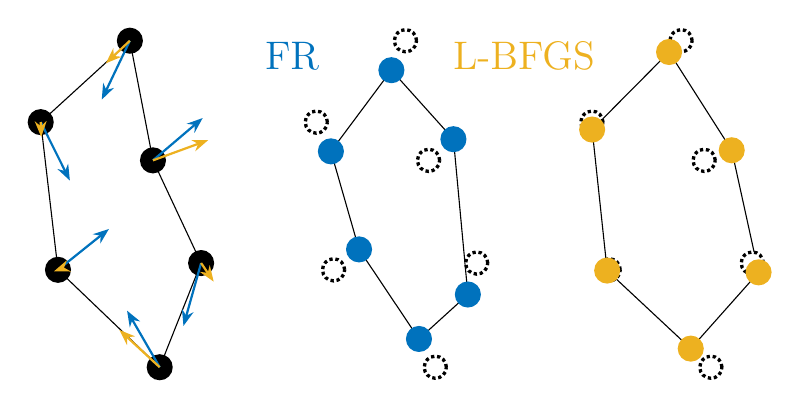
\begin{tikzpicture}
  \foreach \i/\ya/\xa/\yb/\xb/\yc/\xc in {
  % The following data is generated by comparison_FRandLBFGS.py
  0/-1.75626/0.85037/-1.39711/0.643084/-1.51971/0.594647,
  1/-0.519266/-0.441324/-0.25981/-0.117847/-0.528408/-0.466651,
  2/1.35645/-0.660642/0.985416/-0.47547/1.26239/-0.657556,
  3/2.39049/0.471616/2.01626/0.292993/2.24708/0.319419,
  4/0.870969/0.764974/1.13976/1.08073/0.999081/1.11524,
  5/-0.433164/1.37621/-0.832398/1.26411/-0.551213/1.45611
  } {
  % \draw[cA,thick,densely dotted] (3.5+\xa,\ya) -- (3.5+\xb,\yb);
  % \draw[cB,thick,densely dotted] (7+\xa,\ya) -- (7+\xc,\yc);
  \draw[very thick,densely dotted,fill=white] (3.5+\xa,\ya) circle (4pt);
  \draw[very thick,densely dotted,fill=white] (7+\xa,\ya) circle (4pt);

  \coordinate (va\i) at (\xa,\ya);
  \coordinate (vb\i) at (3.5+\xb,\yb);
  \coordinate (vc\i) at (7+\xc,\yc);
  \node[circle, fill=black, minimum size=8pt] at (va\i) {};
  \node[circle, fill=cA, minimum size=8pt] at (vb\i) {};
  \node[circle, fill=cB, minimum size=8pt] at (vc\i) {};

  \draw[cA,thick,-{Stealth[length=2mm]}] (va\i) -- (2*\xb-\xa,2*\yb-\ya);
  \draw[cB,thick,-{Stealth[length=2mm]}] (va\i) -- (2*\xc-\xa,2*\yc-\ya);
  }
  \begin{scope}
    \pgfonlayer{background}
    \foreach \i [count=\j from 1] in {0,1,2,3,4} {
        \draw (va\i) -- (va\j);
        \draw (vb\i) -- (vb\j);
        \draw (vc\i) -- (vc\j);
      }
    \draw (va5) -- (va0);
    \draw (vb5) -- (vb0);
    \draw (vc5) -- (vc0);
    \endpgfonlayer
  \end{scope}

  \node[cA,anchor=east] at (3.0,2.2) {\Large{FR}};
  \node[cB,anchor=east] at (6.5,2.2) {\Large{L-BFGS}};
\end{tikzpicture}
\end{document}
